\documentclass[11pt,journal]{article}
%\usepackage{hyperref}
%\usepackage[breaklinks]{hyperref}
\usepackage{breakurl}
\usepackage{url}
\usepackage{listings}
\usepackage{courier}
\usepackage{amsmath}
\usepackage{graphicx}
\graphicspath{ {/home/agata/Documents/coursework/HPC/assign2/} }
%\ifCLASSOPTIONcompsoc
% IEEE Computer Society needs nocompress option
% requires cite.sty v4.0 or later (November 2003)
\usepackage[nocompress]{cite}

%\else
% normal IEEE
\usepackage{cite}
%\fi

\hyphenation{op-tical net-works semi-conduc-tor}
\addtolength{\oddsidemargin}{-.875in}
\addtolength{\evensidemargin}{-.875in} 
\addtolength{\textwidth}{1.75in}

\addtolength{\topmargin}{-.875in}
\addtolength{\textheight}{1.75in}
\newcommand\tab[1][1cm]{\hspace*{#1}}
\begin{document}
	\title{High Performance Computing, Assignment 2}
	
	\author{UID: 1690550}% <-this % stops a space
		%\protect\\
		%\thanks{}}
	
	% The paper headers



	% IEEEtran.cls defaults to using nonbold math in the Abstract.
	% This preserves the distinction between vectors and scalars. However,
	% if the journal you are submitting to favors bold math in the abstract,
	% then you can use LaTeX's standard command \boldmath at the very start
	% of the abstract to achieve this. Many IEEE journals frown on math
	% in the abstract anyway. In particular, the Computer Society does
	% not want either math or citations to appear in the abstract.
	
	% Note that keywords are not normally used for peerreview papers.
	
	% make the title area
	\maketitle
	
	
	% To allow for easy dual compilation without having to reenter the
	% abstract/keywords data, the \IEEEcompsoctitleabstractindextext text will
	% not be used in maketitle, but will appear (i.e., to be "transported")
	% here as \IEEEdisplaynotcompsoctitleabstractindextext when compsoc mode
	% is not selected <OR> if conference mode is selected - because compsoc
	% conference papers position the abstract like regular (non-compsoc)
	% papers do!
	%\IEEEdisplaynotcompsoctitleabstractindextext
	% \IEEEdisplaynotcompsoctitleabstractindextext has no effect when using
	% compsoc under a non-conference mode.
	
	
	% For peer review papers, you can put extra information on the cover
	% page as needed:
	% \ifCLASSOPTIONpeerreview
	% \begin{center} \bfseries EDICS Category: 3-BBND \end{center}
	% \fi
	%
	% For peerreview papers, this IEEEtran command inserts a page break and
	% creates the second title. It will be ignored for other modes.
	%\IEEEpeerreviewmaketitle
	\section{Initial readings, before any changes were made}
	After a clean make and running the code for the first time, we get the following results from gprof:
	\begin{table}[h]
		\centering
		\begin{tabular}{c|c}
			function & 1  \\
			\hline
			poisson & 23.14 \\
			compute\_tentative\_velocity & 1.10 \\
			compute\_rhs & 0.12 \\
			apply\_boundary\_conditions & 0.02 \\
			set\_timestep\_interval & 0.02 \\
			update\_velocity & 0.02\\
		\end{tabular}
	\end{table}

	We can see that the poisson function is by far the most expensive one, and so we shall focus on it first.
	
	\section{MPI approach}
	\subsection{Domain Decomposition}
	
	We have the option to decompose the region in 1 or 2 directions. After some trial and error, we find that attempting to split the region both horizontally and vertically is not very helpful. It creates a lot of problems for communication between processes later, and generally we do not get much improvement this way. Additionally we can observe that the data is contiguous in columns, but not in rows.
	
	\begin{figure}[h]
		\centering
		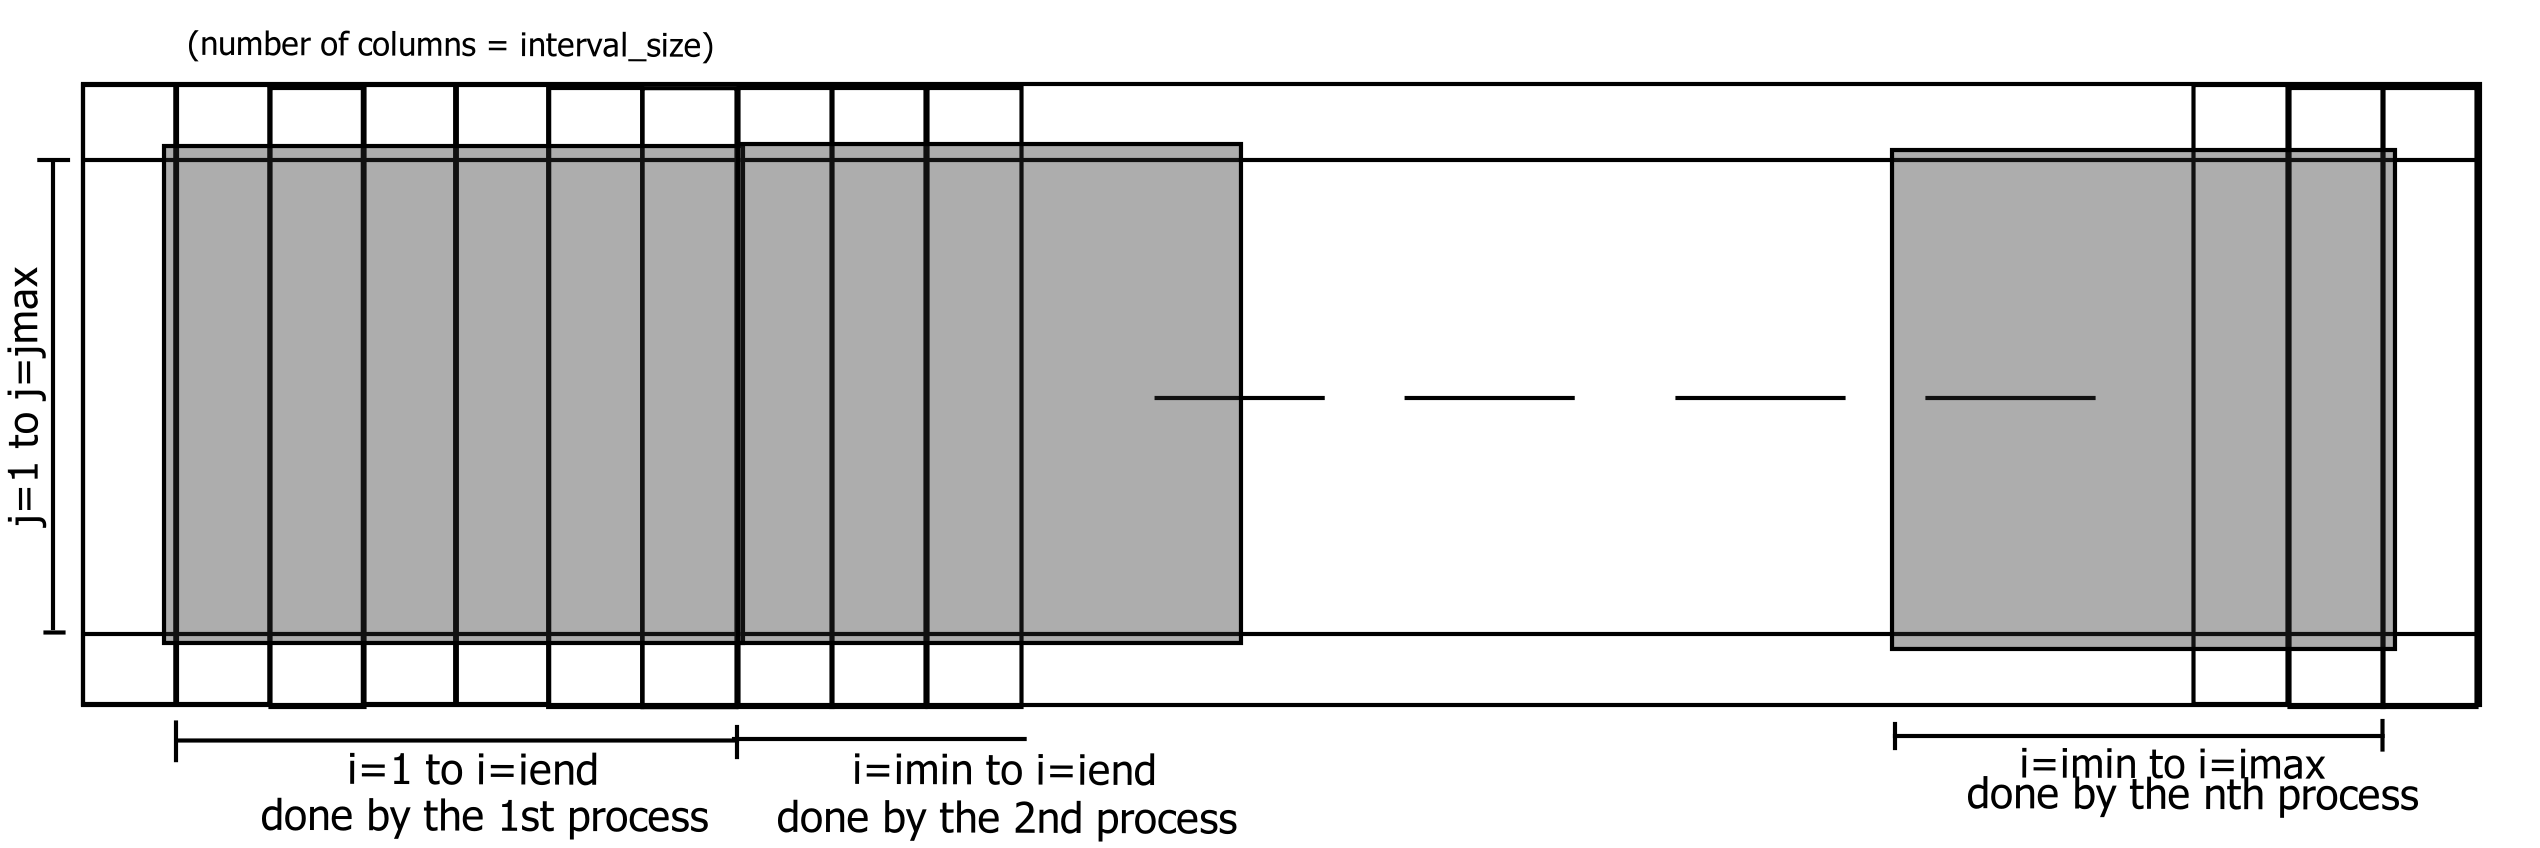
\includegraphics[scale=0.6]{HPC_diag1.png}
		\caption{Domain decomposition}
	\end{figure}
	Therefore we split the region into vertical chunks, one for each process, as shown in Fig. 1. It is straightforward to calculate the number of chunks necessary. We can find the number of processes using:\\
	\tab\\
	\tab \texttt{int nprocs = 0}\\
	\tab \texttt{MPI\_Comm\_size(MPI\_COMM\_WORLD, \&nprocs);}
	
	We put that right after initializing MPI and working out number of processes and assigning task ids, just above the main loop. For ease of calculations, we allow only a number of processes by which the size of the array is divisible. Otherwise we would get uneven chunks.
	
	Each process is assigned a chunk consisting of $interval\_size = \frac{imax}{nprocs} $ columns to balance the load.
	
	We had to define new variables, imin and iend to denote the first and the last column of a chunk respectively. They were added as parameters to each function in 'simulation.c' (and its header).
	
	\subsection{Passing boundaries}
	The processes have to exchange boundaries with their neighbours. It is done by passing the column imin to the neighbour process on the left, and iend to the neighbour on the right. Of course the 1st and last process have only a single neighbour, so to exchange boundaries we use the following:
	\texttt{\\
	\tab if (proc != nprocs -1) \{  \\
	\tab \tab MPI\_Send(\&p[iend], jmax+2, MPI\_FLOAT, proc+1, 0, MPI\_COMM\_WORLD);\\
	\tab \tab MPI\_Recv(\&p[iend+1], jmax+2, MPI\_FLOAT, proc+1, 1, MPI\_COMM\_WORLD);\\
	\tab \}
	}

	Similarly for a process to the left, if the process isn't 0, we send column imin, and receive imin-1. This is pictured in Fig. 2.
	\begin{figure}[h]
		\centering
		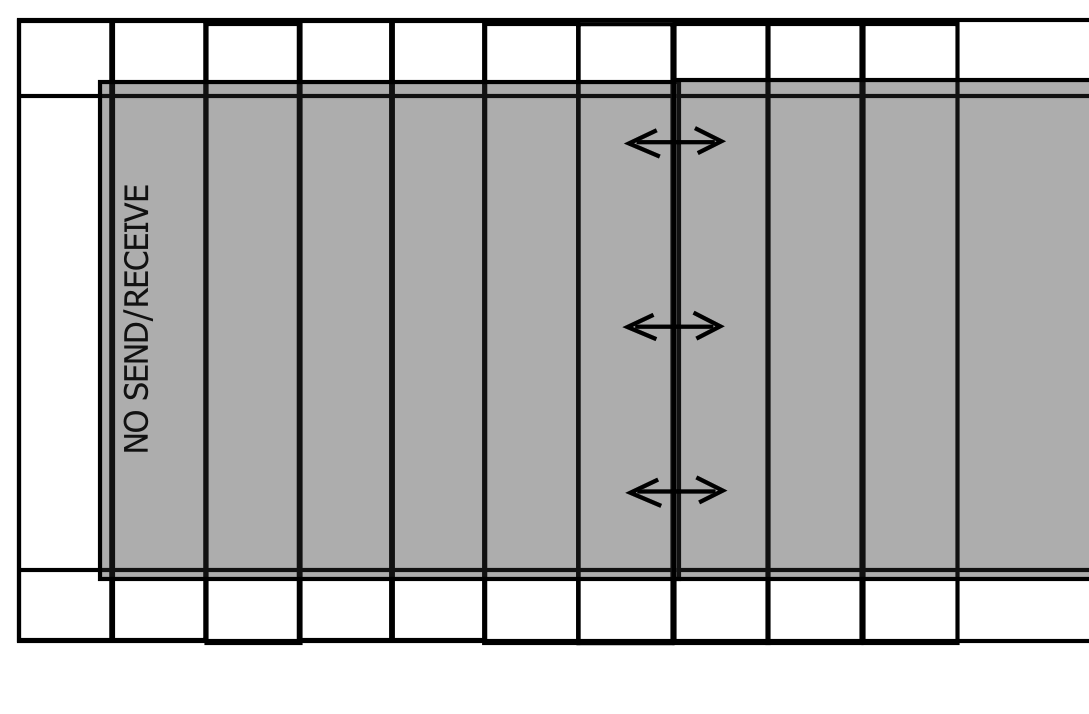
\includegraphics[]{HPC_diag2.png}
		\caption{Boundary sharing}
	\end{figure}	
	
	\subsection{Reductions}
	There are a few places where reductions need to take place, and they are easy to miss. In each case we create a copy of the variable (naming convention: var\_global), to reduce to.
	 \begin{itemize}
	 	\item In poisson() function: p0 is the sum of squares of the values in p. We need MPI\_SUM.
	 	\item In poisson() function: *res is a more complicated function, so we create a temporary variable and a global version of the latter. Later we can calculate *res using temp\_global
	 	\item In set\_timestamp\_interval() function, both umax and vmax can be reduced with MPI\_MAX.
	 \end{itemize}
 

	
	\subsection{Gathering the data}
	After the main loop, we need to gather matrices p, u, and v, which are then printed to a file by the MASTER process. It is most efficient to do it in place. We also put an \texttt{MPI\_Barrier} before gathering, to ensure that the processes have finished their calculations.
	
	We elected to use \texttt{MPI\_Gatherv}. It requires defining our data pattern. Since we want to gather it on the MASTER process (process 0), we stop it from sending anything to itself, by defining first data chunk to be of size 0 and the following ones of (number of columns in each chunk) $\times$ (jmax+2). The displacement in each case is just the size of the chunk after the previous one.
	
	To avoid creating a copy of the array, which would be slower and memory inefficient, we use \texttt{MPI\_IN\_PLACE} as the parameter for the receiving buffer. 

	Other than the main loop, there is one more place where gathering data has to happen - at the end of update\_velocity() function, output of which is used to apply boundary conditions.
	
	Before each MPI\_Gatherv statement, we put a barrier to make sure that all processes have finished their calculations by then.
	
	\subsection{Results}
	\pagebreak
	\section{Using OpenMP}
	First we observe that in the \texttt{simulation.c} there are multiple loops, however not all of them may be worth parallelising.  
	

	% that's all folks
\end{document}

